\documentclass[12pt, oneside]{book}  
\usepackage[T1]{fontenc}   
\usepackage[utf8]{inputenc}  
\usepackage{microtype}  
\usepackage[sc]{mathpazo}  
\usepackage{hyperref}  
\usepackage{charter}
\hypersetup{
	colorlinks=true,  % Links appear in color
	linkcolor=black,   % Color for internal links
	citecolor=blue,   % Color for citations
	urlcolor=blue     % Color for URLs
}
\usepackage{amsmath}
\usepackage{enumitem}
\usepackage{amsmath, amssymb, amsthm}  
\usepackage[a4paper, margin=1in]{geometry}
\usepackage{booktabs}  
\usepackage{array} 
\usepackage{graphicx}
\usepackage{caption}
\usepackage{float}
\usepackage[backend=biber,style=apa]{biblatex}
\addbibresource{references.bib}
\usepackage{fancyhdr}
% Page layout configuration
\geometry{a4paper, margin=1in}

% Fancyhdr configuration for headers and footers
\pagestyle{fancy}
\fancyhead[L]{\nouppercase{\leftmark}}
\fancyhead[R]{\nouppercase{\rightmark}}
\fancyfoot[C]{\thepage}
\usepackage{xcolor} 
\definecolor{myblue}{RGB}{0, 102, 204}
\usepackage{listings}

\lstset{
	basicstyle=\ttfamily\small,   % Font style for the code (typewriter font, small size)
	breaklines=true,              % Automatically break lines that are too long
	commentstyle=\color{gray},    % Style for comments
	keywordstyle=\color{blue},    % Style for keywords
	stringstyle=\color{red},      % Style for strings
	numbers=left,                % Line numbers on the left
	numberstyle=\tiny,           % Style for line numbers
	stepnumber=1,                % Number every line (1 = every line, 2 = every second line, etc.)
	backgroundcolor=\color{lightgray}, % Background color for code blocks
	captionpos=b,                % Position of the caption (b = bottom, t = top)
	escapeinside={(*@}{@*)},     % Escape to LaTeX within code (useful for adding LaTeX commands)
	morecomment=[s][\color{magenta}]{/*}{*/}, % Additional comment style
}
\usepackage{tocbibind}
\usepackage{titlesec}
\usepackage{makeidx}
\makeindex

% Title and author
\title{{\Huge Data's DNA}}
\author{{\LARGE Mahdi}}
\date{{\large \today}}

\begin{document}
	\frontmatter
	\mainmatter
	\maketitle
	\tableofcontents
\chapter{OBJECTIVES}

The purpose of this book is to serve as a comprehensive guide and reference for learning about data and data types in programming and computer science. The objectives of this book are:

\begin{itemize}
	\item To provide an in-depth understanding of the nature of data, its theoretical foundations, and its role in modern technology.
	\item To explore various data types used in programming, from primitive to advanced types, and their importance in software development.
	\item To explain the mathematical and theoretical principles related to data, including concepts from information theory and computer science.
	\item To present practical examples and case studies that demonstrate how data is represented, manipulated, and utilized in real-world applications.
	\item To provide a structured and detailed learning path for self-study, aimed at anyone seeking to gain a deep understanding of data types in programming.
\end{itemize}

This book collects content from a variety of online resources, books, articles, and academic papers. Each section or paragraph may include links or references to the original sources used. This approach is intended to compile the best available knowledge, making it easier to learn and understand complex topics in data and programming.

\vspace{0.5cm}
\textbf{Note:} This book is a self-learning project. The content within is curated for personal educational purposes. Some sections may be directly copied from original sources, with the appropriate links or references provided at the end of each section to acknowledge the original authors.

\chapter{INTRODUCTION}

Data is the cornerstone of the digital age, and understanding how data is represented, stored, and manipulated is essential for anyone studying computer science, programming, or related fields. The modern world is driven by data — from everyday applications like social media and search engines to cutting-edge technologies such as artificial intelligence and blockchain.

This book delves into the fundamental concepts of data and data types, starting from their basic definitions to advanced structures and theoretical underpinnings. It is structured to take readers from the preliminary stages of understanding what data is, to exploring its role in algorithms, communication systems, and emerging technologies.

Key themes covered in this book include:
\begin{itemize}
	\item Theoretical foundations of data, including information theory and Shannon's entropy.
	\item The distinction between different types of data, such as structured, unstructured, and semi-structured data.
	\item Primitive and advanced data types used in programming languages, from integers and floats to complex data structures like graphs and trees.
	\item The role of data in algorithms, computation, and software development.
	\item Mathematical models for representing data and the implications of different storage mechanisms.
\end{itemize}

By the end of this book, readers should have a strong conceptual understanding of how data works within the field of computer science and be able to apply this knowledge in practical programming scenarios.

\vspace{0.5cm}
\textbf{Note:} All information and explanations provided in this book are based on a variety of sources, with full credit given to the original authors where applicable. The goal is to provide a clear and concise learning path, and all external material will be properly referenced to avoid confusion.

\chapter{The Nature of Data}
\section{What is Data}
The term 'data' originates from the Latin word *datum*, meaning "something given." Over time, the word has evolved to encompass various definitions, depending on the context in which it is used. In general, data refers to information or facts that can be used for analysis, reasoning, or computation. Below are some well-recognized definitions from different perspectives:\\
\subsection{Definitions of Data}
\subsubsection{Linguistic Origins and Basic Definitions}
According to Webster's Third New International Dictionary, data is "something given or admitted; facts or principles granted or presented; that upon which an inference or argument is based, or from which an ideal system of any sort is constructed." This definition emphasizes the foundational nature of data, implying that data is the starting point for any logical process, whether in science, philosophy, or everyday reasoning.\\\\
Similarly, the Oxford Encyclopaedic English Dictionary defines data as "known facts or things used as a basis for inference or reckoning." This stresses the use of data as input for making judgments, calculations, or conclusions.\\\\
Though 'data' is the plural form of 'datum', it is commonly treated as a singular noun in modern language. While the plural form is technically correct, the singular usage is widely accepted. For consistency in this book, 'data' will be treated as a plural noun, referring to multiple pieces of information or facts.\\
\subsubsection{Definitions from Various Disciplines}

Different fields and organizations have their own definitions of data:

\paragraph{UNESCO's Definition:} 
The United Nations Educational, Scientific and Cultural Organization (UNESCO) defines data as "facts, concepts, or instructions in a formalized manner suitable for communication, interpretation, or processing by human or automatic means." This highlights that data must be structured or organized to be useful, especially in the context of computer systems where data is processed and transferred.\\
\paragraph{Commerce Perspective:}
Robert A. Arnold, in his work *Modern Data Processing*, provides a definition of data in the context of business and accounting, focusing on its role in the management and processing of information relevant to business functions.\\
\paragraph{Economics Perspective:}
The *Dictionary of Modern Economics* describes data as "observations on the numerical magnitude of economic phenomena such as national income, unemployment, or the retail price." In economics, data usually refers to quantifiable measurements or observations that are used to analyze economic trends and make informed decisions.\\
\paragraph{Scientific Definition:}
In the sciences, data is often described as a set of "numerical or qualitative values derived from scientific experiments." According to the *McGraw-Hill Encyclopedia of Science and Technology*, this data is the result of observation and experimentation, and it forms the basis of scientific knowledge.\\
\paragraph{CODATA's Definition:}
The Committee on Data for Science and Technology (CODATA) defines data as the "crystallized presentation of the essence of scientific knowledge in the most accurate form." This implies that scientific data is a refined and exact representation of reality, critical for making advancements in scientific research.\\
\paragraph{Social Sciences Definition:}
In social sciences, data is defined as values or facts, often accompanied by study designs, code books, and research reports, which are used by researchers for secondary analysis. In fields such as sociology and political science, data can be qualitative (like interviews and surveys) or quantitative (like public opinion polls).\\
\paragraph{Humanities Definition:}
In the humanities, data often takes the form of text, such as Biblical materials or Shakespearean drama. The finite amount of text represents a fixed quantity of data, which scholars interpret. However, interpretations can vary widely due to differing viewpoints, even though the text itself remains unchanged. In this sense, humanities data is more subjective and open to different perspectives.\\
\paragraph{Information Science Definition:}
In information science, Shuman (1975) defines data as "quantitative facts derived from experimentation, calculation, or direct observation." Shuman further explains that a more meaningful definition of data is "the symbolization of knowledge," meaning that data represents a raw form of knowledge that must be processed and interpreted to extract meaning.\\
\subsection{Attributes of Data}
Data, regardless of the field it comes from, shares several core attributes:
\begin{itemize}
	\item \textbf{Clarity and Accuracy:} As noted in the CODATA definition, scientific data must be both clear and accurate, meaning it should be easily understandable and precisely represent the phenomenon being measured.
	\item \textbf{Relevance and Arrangement:} Data is only useful when it is relevant to a particular context. It must be organized or structured in a way that allows it to be processed or interpreted effectively.\\
	\item \textbf{Quantitative vs. Qualitative:} Data can be either numerical (quantitative) or descriptive (qualitative). While numerical data allows for more precise analysis, qualitative data often provides deeper insights into complex issues.\\
	\item \textbf{Expanding Nature of Scientific Data:} In sciences, data is not fixed and is continuously expanding as scientists make new observations and use instruments to generate more systematic data.
\end{itemize}
\subsection{Contextual Use of Data}
\subsubsection{Data in Different Domains}
\paragraph{Sciences:} In scientific research, data is often collected through observation and experimentation. Scientists use instruments and measurement tools to record quantitative or qualitative values. As scientific knowledge grows, so does the body of available data.\\
\paragraph{Social Sciences:} In fields such as sociology, economics, and political science, data may include survey results, statistical figures, or observations from field research. Researchers use this data to analyze societal trends and test hypotheses.\\
\paragraph{Humanities:} In disciplines like literature, history, and philosophy, data might consist of texts, documents, or artifacts. The analysis of this data typically involves interpretation and critical thinking, as opposed to statistical analysis.\\
\subsubsection{Symbolization of Knowledge}
Data, in its raw form, lacks meaning until it is processed and interpreted. In information science, the term "symbolization of knowledge" refers to how data must be contextualized and understood within a specific framework to gain relevance and coherence. This is particularly true in fields where data is used to draw conclusions or make predictions.\\
\subsection{The Expanding Role of Data}
In the modern digital era, data is expanding at an unprecedented rate due to advancements in technology, including the proliferation of internet usage, artificial intelligence, and big data analytics. As a result, data has become a valuable resource for decision-making, innovation, and economic development.
\vspace{0.5cm}\\
\textbf{Note:} The definitions and explanations in this section are collected from various authoritative sources. Full references to these sources are provided to acknowledge the original authors. For further reading, you can access the full text at the following link: \\
 \href{https://egyankosh.ac.in/bitstream/123456789/10935/3/Unit-2.pdf}{UNESCO - The Nature of Data (PDF)}.

\section{Theoretical Foundations of Data}

\subsection{Data in Information Theory}
According to \textit{Merriam-Webster} (merriam-webster.com), “Information is any entity or form that provides the answer to a question of some kind or resolves uncertainty.” This definition underscores the relationship between data, information, and knowledge: data represents values attributed to various parameters, while knowledge signifies an understanding of real things or abstract concepts. However, modern Information Theory is not a general theory that addresses these relationships directly. Instead, it is a mathematical framework designed to model and analyze how information is transmitted and processed.\\
The foundation of Information Theory can be traced back to Claude E. Shannon's groundbreaking article, “A Mathematical Theory of Communication,” published in the Bell System Technical Journal in 1948. This work laid the groundwork for understanding how messages can be accurately transmitted over communication channels. As Shannon stated in the introduction of his article:\\
\begin{quote}
	“The fundamental problem of communication is that of reproducing at one point either exactly or approximately a message selected at another point. Frequently the messages have meaning. . . . These semantic aspects of communications are irrelevant to the engineering problem. . . . The system must be designed to operate for each possible selection, not just the one which will actually be chosen since this is unknown at the time of design.”
\end{quote}
In 1964, Shannon, along with Warren Weaver, published a book titled “The Mathematical Theory of Communication,” which further emphasized the general applicability of his theories beyond just communication systems. This work solidified the importance of Information Theory in understanding various phenomena in multiple disciplines.\\
Information Theory provides essential methods and analytical tools for designing effective communication systems. Figure \ref{fig:1.1} illustrates the basic components of a communication system, highlighting the key elements involved in the process of transmitting information:\\
\begin{figure}[h!]
	\centering
	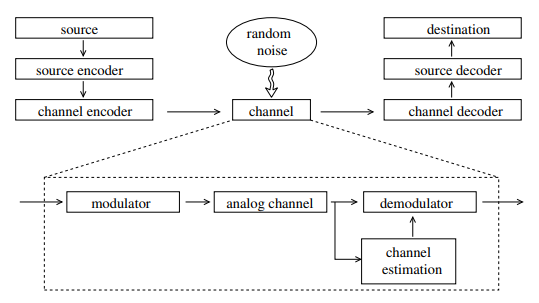
\includegraphics[width=\linewidth]{./1.1.png}
	\caption{The general model of a communication system.}
	\label{fig:1.1}
	\textbf{Components:}
\end{figure}
\\
\begin{itemize}
	\item \textbf{Source}: This is where the information originates. It can be any type of data, such as text, audio, or video. For instance, a text document or a video file could serve as the source.
	\item \textbf{Source Encoder}: The source encoder transforms the information from the source into a suitable format for transmission. This may involve compressing the data to reduce its size, making it more efficient to send. For example, a text file might be compressed into a smaller file format like ZIP.
	\item \textbf{Channel Encoder}: This component adds redundancy to the encoded message to protect against errors that may occur during transmission. The redundancy helps the system detect and correct errors. For example, adding parity bits to the data stream can help identify if any bits were altered during transmission.
	\item \textbf{Channel}: The channel is the medium through which the encoded message travels. It can be a physical medium like copper wires or fiber optics, or a wireless medium such as radio waves.
	\item \textbf{Random Noise}:  Noise represents unwanted disturbances that can interfere with the transmitted signal. This could be caused by electrical interference, weather conditions, or other environmental factors. 
	\item \textbf{Channel Decoder}:  This component attempts to correct any errors that occurred during transmission by using the redundancy added by the channel encoder. For instance, it checks the parity bits and makes corrections if discrepancies are found.
	\item \textbf{Demodulator}: The demodulator converts the modulated signal back into its original format after it has traveled through the channel. For example, it might convert a radio signal back into a digital signal.
	\item \textbf{Analog Channel}:  In some systems, the channel might be an analog medium, which requires modulation to convert the digital signals into an analog format suitable for transmission.
	\item \textbf{Channel Estimation}: This process involves estimating the characteristics of the channel to improve the accuracy of the received signal. It helps in adjusting the decoding process based on the estimated conditions of the channel.
	\item \textbf{Source Decoder}:  Finally, the source decoder takes the corrected signal and converts it back into a format that the destination can use, such as a readable text file or a playable audio file.
	\item \textbf{Destination}:  The destination is the final recipient of the transmitted message. This can be a device, user, or system that processes the received information, such as a computer, smartphone, or any device capable of interpreting the data.
\end{itemize}
\subsubsection*{Example of Transmitting a Text Message}

Let's consider a straightforward example of how a text message is transmitted using the communication system.

\subsubsection*{Example Scenario}
\textbf{Source}: A user types the message "Hello, World!" on their computer.

\subsubsection*{Step-by-step Process}

\begin{enumerate}[label=\arabic*.]
	\item \textbf{Source}: 
	The original message is: 
	\[\text{Message} = "Hello, World!"\]
	\item \textbf{Source Encoder}: 
	The message is encoded and compressed, resulting in a smaller representation, saved as:
	\[\text{Encoded Message} = \text{Helloworld.txt}\]
	\item \textbf{Channel Encoder}: 
	Redundant data, such as parity bits, are added to the encoded message for error detection. This can be represented as:
	\[	\text{Channel Encoded Message} = \text{Helloworld.txt + Parity Bits}\]
	\item \textbf{Channel}: 
	The encoded message is transmitted through a wireless channel (e.g., Wi-Fi):
	\[\text{Channel} \rightarrow \text{Helloworld.txt + Parity Bits}\]
	\item \textbf{Random Noise}: 
	During transmission, interference introduces noise, causing the message to become distorted:
	\[\text{Received Message} = "Helo, World!" \]
	
	\item \textbf{Channel Decoder}: 
	The receiver uses the redundancy (parity bits) to detect and correct the error:
	\[\text{Corrected Message} = "Hello, World!"\]
	
	\item \textbf{Demodulator}: 
	The received signal is demodulated back into its original digital format.
	
	\item \textbf{Source Decoder}: 
	The corrected message is decoded to restore the original text format:
	\[\text{Final Message} = "Hello, World!"\]
	
	\item \textbf{Destination}: 
	The user receives the corrected message on their computer.
\end{enumerate}
\\While the origins of Information Theory are rooted in electrical engineering and telecommunications, its principles have proven invaluable in modeling phenomena across various fields, including physics, mathematics, statistics, computer science, and economics. It cannot simply be regarded as a subset of communication theory; it encompasses a broader scope of applications.\vspace{0.5cm}\\
\textbf{Note:} The definitions and explanations in this section are collected from various authoritative sources. Full references to these sources are provided to acknowledge the original authors. For further reading, you can access the full text at the following link: \\
\href{https://www.ti.rwth-aachen.de/teaching/InformationTheory/ws1819/data/InformationTheory.pdf}{Information Theory (PDF)}.

\subsubsection{Quantifying Data: Bits, Bytes, and Beyond}
Data, in its most basic form, can be quantified using bits (binary digits) and bytes. A bit is the smallest unit of data, representing a binary state (0 or 1), while a byte typically consists of 8 bits. This subsection explains how larger units of data, such as kilobytes (KB), megabytes (MB), gigabytes (GB), and beyond, are derived from these basic units, as well as their relevance in digital storage and communication.

\subsubsection{Shannon's Entropy and Information Content}
Shannon's entropy is a fundamental concept in information theory that quantifies the uncertainty or unpredictability in data. It is a measure of the information content in a message and helps in understanding how much data can be compressed. This subsection explains how entropy relates to data transmission, compression, and the efficient encoding of information.

\subsubsection{Noise, Redundancy, and Compression in Data}
In communication systems, noise refers to random disturbances that can alter data during transmission. Redundancy is often added to data to counteract noise and improve accuracy. Compression techniques reduce the amount of data by eliminating unnecessary redundancy. This subsection covers how these concepts affect the integrity and efficiency of data in communication channels.

\subsubsection{Data Transmission and Loss in Communication Systems}
Data loss can occur due to various factors such as noise or interruptions in communication systems. This subsection examines how data is transmitted across networks and the mechanisms used to detect and correct errors, ensuring that the transmitted data remains intact.

\subsection{Data in Computer Science}
This section covers how data is viewed and used in the field of computer science, focusing on historical perspectives, different types of data, and the role of data in algorithms and computational processes.

\subsubsection{Historical Perspectives on Data Representation}
Historically, data representation has evolved from simple binary codes to more complex formats like ASCII, Unicode, and structured data formats (e.g., JSON, XML). This subsection explores the history of data representation, including early coding systems and their impact on computing.

\subsubsection{Symbolic Data vs Numerical Data}
Data in computer science is categorized as symbolic (representing concepts or entities, such as words or letters) or numerical (representing quantitative values, such as integers or floating-point numbers). This subsection discusses the differences between these two types of data and their applications in computing.

\subsubsection{Data in the Context of Algorithms and Computation}
In algorithms, data is the input that is processed to produce an output. This subsection explains the role of data in computational processes, including sorting, searching, and data transformation algorithms. It also highlights how algorithms operate on data to solve problems efficiently.

\subsubsection{Data as Input/Output in Turing Machines}
A Turing machine, a theoretical model of computation, uses data as both input and output during its operations. This subsection explores how data is handled within the Turing machine model, which forms the foundation of modern computation theory.

\subsection{Data as an Abstract Entity}
This section delves into philosophical and theoretical frameworks that treat data as an abstract entity, examining its role in knowledge representation, mathematical structures, and modeling.

\subsubsection{Philosophical Perspectives on Data and Knowledge}
Data is often considered the raw material for knowledge. This subsection explores philosophical views on the relationship between data, information, and knowledge, addressing questions such as whether data can exist independently of interpretation and how it contributes to human understanding.

\subsubsection{Mathematical Structures of Data: Sets, Graphs, and Trees}
Data can be represented in abstract mathematical structures such as sets (unordered collections), graphs (networks of nodes and edges), and trees (hierarchical structures). This subsection explains how these structures are used to model and organize data in various fields, from computer science to data science.

\subsubsection{Data and Models in Theoretical Frameworks}
Theoretical frameworks in fields like machine learning and statistics rely on models that are built from data. This subsection explores how data is used to create and validate models, including mathematical and statistical models, and how these models represent the underlying patterns and relationships in the data.

===

\section{The Relationship Between Data and Information}
\subsection{Data vs Information}
\subsubsection{Definitions and Distinctions}
\subsubsection{The Transformative Process from Data to Information}
\subsection{Data, Information, and Knowledge Hierarchy}
\subsubsection{The DIKW Pyramid}
\subsubsection{Knowledge Representation and Data}
\subsection{Data Lifecycle}
\subsection{Data Creation and Collection}
\subsubsection{Methods of Data Collection: Surveys, Sensors, and Logs}
\subsubsection{Data Quality and Accuracy Considerations}
\subsection{Data Storage and Processing}
\subsubsection{Data Formats: CSV, JSON, XML}
\subsubsection{Data Storage Solutions: SQL vs NoSQL}
\subsection{Data Analysis and Interpretation}
\subsubsection{Descriptive and Inferential Statistics}
\subsubsection{Data Visualization Techniques}
\subsection{Data Archiving and Disposal}
\subsubsection{Data Retention Policies}
\subsubsection{Ethics in Data Disposal}

\chapter{Fundamental Concepts of Data Types}
\section{Mathematical Foundations of Data Types}
\subsection{Set Theory and Data Types}
\subsubsection{Sets as Fundamental Structures in Data Representation}
\subsubsection{Operations on Sets: Union, Intersection, and Cartesian Products}
\subsubsection{Finite and Infinite Sets in Data Theory}
\subsubsection{Multisets and Their Applications in Data Representation}
\subsection{Algebraic Data Types (ADTs)}
\subsubsection{Sum Types, Product Types, and Recursive Types}
\subsubsection{Pattern Matching in Algebraic Data Types}
\subsubsection{Examples of ADTs in Functional Programming}
\subsubsection{Proofs and Data Integrity in ADTs}
\subsection{Type Theory in Programming Languages}
\subsubsection{Lambda Calculus and Data Representation}
\subsubsection{Typed vs Untyped Lambda Calculus: A Comparative Study}
\subsubsection{Type Systems and Soundness in Programming Languages}

\section{Data Types as Abstractions}
\subsection{Type Abstractions and Modular Programming}
\subsubsection{Abstract Data Types (ADTs) vs Concrete Data Types}
\subsubsection{The Role of Interfaces and Abstract Classes}
\subsubsection{Practical Applications: Abstraction in Large-Scale Systems}
\subsection{Data Types in Compilation and Interpretation}
\subsubsection{Role of Types in Parsing and Compilation Phases}
\subsubsection{How Compilers Enforce Type Safety and Error Handling}
\subsubsection{Dynamic vs Static Type Systems: Efficiency and Flexibility}
\subsection{Memory Management and Data Types}
\subsubsection{Data Types and Garbage Collection Mechanisms}
\subsubsection{Stack vs Heap Allocation: Performance Implications}
\subsubsection{Memory Leaks and Type Safety}

\section{Categories of Data Types}
\subsection{Primitive vs Non-Primitive Data Types}
\subsubsection{Atomic Data Types: Integers, Floats, and Booleans}
\subsubsection{Composite Data Types: Arrays, Structs, and Objects}
\subsubsection{Dynamic Data Types: Lists, Queues, and Stacks}
\subsubsection{Complex Data Types: Maps, Sets, and Hash Tables}
\subsection{Data Types as Logical Models of Data}
\subsubsection{Logical Programming and Data Types in Prolog}
\subsubsection{Formal Models of Data Structures in Logic Programming}
\subsection{Finite and Infinite Data Types}
\subsubsection{Finite Data Structures in Practical Applications}
\subsubsection{Streams and Lazy Evaluation in Infinite Data Types}

\chapter{Data Types in Formal Computer Science}
\section{Formal Definitions and Properties of Data Types}
\subsection{Data Types as Mathematical Objects}
\subsubsection{Formal Set Definitions of Data Types}
\subsubsection{Algebraic Structures: Monoids, Groups, and Rings}
\subsubsection{Operations on Data Types: Homomorphisms and Isomorphisms}
\subsection{Domain Theory in Data Types}
\subsubsection{Complete Partial Orders and Continuous Data Types}
\subsubsection{Domains in Programming Language Semantics}
\subsubsection{The Fixed-Point Theorem and Recursive Data Types}
\subsection{Lattice Theory and Type Hierarchies}
\subsubsection{Lattices in Type Systems: Formal Definitions}
\subsubsection{Subtype Polymorphism and Inheritance in Type Lattices}

\section{Type Systems and Type Checking}
\subsection{Formal Semantics of Type Systems}
\subsubsection{Operational, Denotational, and Axiomatic Semantics}
\subsubsection{Formal Type Systems and Their Proofs}
\subsection{Static vs Dynamic Type Systems}
\subsubsection{Trade-offs Between Static and Dynamic Typing in Programming Languages}
\subsubsection{Type Inference Algorithms: Hindley-Milner and Beyond}
\subsection{Type Safety and Soundness Theorems}
\subsubsection{Understanding Type Safety in Programming Languages}
\subsubsection{Formal Proofs of Type Soundness}
\subsubsection{Examples of Type Safety Violations in Real-World Programs}

\section{Data Type Completeness and Expressiveness}
\subsection{Expressiveness of Type Systems}
\subsubsection{Comparing the Expressive Power of Data Types}
\subsubsection{Type Systems in Polymorphic and Higher-Order Languages}
\subsection{Normalization and Termination in Typed Systems}
\subsubsection{Strong Normalization Theorems and Their Applications}
\subsubsection{Proving Termination in Typed Lambda Calculi}
\subsection{Type Isomorphisms and Representation Theorems}
\subsubsection{Understanding Type Isomorphisms in Programming Languages}
\subsubsection{Practical Applications of Representation Theorems in Type Systems}

\chapter{Data Models and Abstractions in Programming}
\section{Mathematical Models of Data}
\subsection{Graphs and Trees as Data Models}
\subsubsection{Graph Theory Basics}
\subsubsection{Tree Traversal Algorithms}
\subsection{Turing Machines and Data Representation}
\subsubsection{Turing Machine Models and Data}
\subsubsection{Applications of Turing Machines in Data Processing}
\section{Data Models in Programming Languages}
\subsection{Declarative vs Imperative Data Models}
\subsubsection{Comparison of Programming Paradigms}
\subsubsection{Examples of Data Models in Declarative Languages}
\subsection{Data Models in Functional Programming}
\subsubsection{First-Class and Higher-Order Functions}
\subsubsection{Data Immutability in Functional Paradigms}
\section{Advanced Data Models}
\subsection{Dataflow Models}
\subsubsection{Overview of Dataflow Programming}
\subsubsection{Examples of Dataflow Languages}
\subsection{Reactive Data Models}
\subsubsection{Understanding Reactivity in Data Models}
\subsubsection{Applications of Reactive Programming}
\subsection{Event-Driven Data Models}
\subsubsection{Event-Driven Architectures and Their Benefits}
\subsubsection{Examples of Event-Driven Systems}

\chapter{Data Types and Algorithms}
\section{Data Types and Algorithm Efficiency}
\subsection{Big-O Complexity and Data Types}
\subsubsection{Understanding Time and Space Complexity}
\subsubsection{Analyzing the Impact of Data Types on Algorithm Efficiency}
\subsubsection{Real-World Case Studies: Efficient Data Type Selection}
\subsection{Impact of Data Structures on Algorithm Performance}
\subsubsection{Complexity of Sorting and Searching Algorithms Based on Data Types}
\subsubsection{Data Types and Asymptotic Performance in Algorithms}
\section{Data Types in Algorithm Design}
\subsection{Algorithmic Techniques for Abstract Data Types}
\subsubsection{Divide and Conquer Techniques in Recursive Data Types}
\subsubsection{Greedy Algorithms and Dynamic Programming}
\subsection{Data Structures and Recursion}
\subsubsection{Recursion vs Iteration in Data Structure Traversals}
\subsubsection{Applications of Recursive Data Structures in Problem Solving}
\section{Optimization Techniques Based on Data Types}
\subsection{Cache Optimization and Data Layout}
\subsubsection{Improving Cache Performance with Data Types}
\subsubsection{Optimizing Data Layout for Cache Locality}
\subsection{Memory Alignment and Data Access Speed}
\subsubsection{Understanding Memory Alignment Constraints}
\subsubsection{Techniques for Optimizing Data Access Speed}

\chapter{Memory and Data Types}
\section{Memory Models and Data Representation}
\subsection{Von Neumann Architecture and Data Representation}
\subsubsection{Components of the Von Neumann Model}
\subsubsection{Data Representation in Memory Architecture}
\subsection{Harvard Architecture vs Modified Harvard}
\subsubsection{Comparative Analysis of Memory Architectures}
\subsubsection{Implications for Data Processing}
\section{Data Alignment and Memory Access}
\subsection{Alignment Constraints}
\subsubsection{Understanding Alignment Requirements}
\subsubsection{Consequences of Misalignment}
\subsection{Impact of Data Types on Memory Usage}
\subsubsection{Memory Overhead and Management}
\subsubsection{Memory Fragmentation Issues}
\section{Data Types and Virtual Memory}
\subsection{Paged Memory Systems}
\subsubsection{Overview of Paging Mechanisms}
\subsubsection{Advantages of Paging in Data Access}
\subsection{Data Type Representation in Virtual Memory}
\subsubsection{Address Translation Mechanisms}
\subsubsection{Performance Considerations in Virtual Memory}
\subsection{Memory Segmentation and Data Boundaries}
\subsubsection{Understanding Segmentation}
\subsubsection{Applications of Segmentation in Data Handling}

\chapter{Type Theories in Modern Programming Languages}
\section{Lambda Calculus and Type Systems}
\subsection{Simply Typed Lambda Calculus}
\subsubsection{Definitions and Basic Concepts}
\subsubsection{Applications of Simply Typed Lambda Calculus}
\subsection{Polymorphic Lambda Calculus}
\subsubsection{System F and Its Implications}
\subsubsection{Polymorphism in Programming Languages}
\subsection{Dependent Types and Programming}
\subsubsection{Understanding Dependent Types}
\subsubsection{Practical Applications of Dependent Types}

\section{Object-Oriented Programming and Data Types}
\subsection{Classes and Objects as Data Types}
\subsubsection{Encapsulation and Data Hiding}
\subsubsection{Inheritance and Polymorphism}
\subsection{Interfaces and Abstract Data Types in OOP}
\subsubsection{Defining Interfaces in Programming Languages}
\subsubsection{Comparison of Interface Implementations}
\section{Functional Programming and Data Types}
\subsection{Immutable Data Types in Functional Languages}
\subsubsection{Understanding Immutability}
\subsubsection{Advantages of Immutable Data Structures}
\subsection{Functional Data Structures and Their Characteristics}
\subsubsection{Examples of Functional Data Structures}
\subsubsection{Performance Implications of Functional Data Types}

\chapter{Data Types in Practical Applications}
\section{Data Types in Database Management Systems}
\subsection{Relational Data Types and SQL}
\subsubsection{Defining Data Types in SQL}
\subsubsection{Normalization and Data Integrity}
\subsection{NoSQL Data Models}
\subsubsection{Understanding Document, Key-Value, and Graph Databases}
\subsubsection{Use Cases for NoSQL Data Models}
\section{Data Types in Web Development}
\subsection{Data Types in JavaScript and JSON}
\subsubsection{JavaScript Data Types and Their Characteristics}
\subsubsection{JSON as a Data Format}
\subsection{Data Types in RESTful APIs}
\subsubsection{Understanding Data Representation in APIs}
\subsubsection{Data Types and Serialization Techniques}
\section{Data Types in Machine Learning and AI}
\subsection{Data Types in Machine Learning Models}
\subsubsection{Data Representation in Feature Engineering}
\subsubsection{Understanding Structured vs Unstructured Data}
\subsection{Data Types and Model Performance}
\subsubsection{Impact of Data Types on Model Accuracy}
\subsubsection{Best Practices for Data Preparation}

\chapter{Future Directions in Data Types and Data Science}
\section{Emerging Data Types in Technology}
\subsection{Big Data and Complex Data Types}
\subsubsection{Understanding Big Data Characteristics}
\subsubsection{Handling Complex Data Structures}
\subsection{Quantum Data Types and Computing}
\subsubsection{Overview of Quantum Computing Principles}
\subsubsection{Implications for Data Representation}
\section{Trends in Data Science and Data Types}
\subsection{The Role of Data Types in AI and Machine Learning}
\subsubsection{Data Types for Training Models}
\subsubsection{Understanding Data Bias and Ethics}
\subsection{Future Challenges in Data Representation}
\subsubsection{Addressing Data Privacy and Security}
\subsubsection{Evolving Standards in Data Management}

\chapter{Conclusion}
\section{Summary of Key Concepts}
\section{Future Perspectives on Data Types}
\section{The Ongoing Evolution of Data Science}


\end{document}